\chapter{Einleitung}
Seitdem Rechner mit Maschinencode programmiert werden, steigt das Abstraktionslevel der Programmiersprachen kontinuierlich an (siehe Abbildung \ref{paradigmnsintime}). Wer die Assemblersprachen kennt und fürchtet, weiß Programmiersprachen wie Fortran, Pascal oder C zu schätzen, da sie Kontrollstrukturen einführen, welche leicht verstanden und eingesetzt werden können. Wer stets wiederkehrende Muster programmiert, bedient sich der Objektorientierten Sprachen, wie zum Beispiel Java oder C++.
Indem die Logik hinter Programmiersprachen den Paradigmen angeglichen werden, die die Menschen intuitiv(oder am einfachsten) beherrschen, wird Programmieren erheblich effizienter, sowohl im Lernprozess, als auch in der Umsetzung. 
Der prozentuale Anteil an wiederverwendbarem Code in einem Projekt steigt mit dem Abstraktionslevel der verwendeten Programmierparadigmen. Code, der wiederverwendet werden kann, spart Zeit und reduziert die Chance neue Fehler in das Projekt einzuarbeiten. Die Objektorientierung wurde eingeführt um wiederkehrende Elemente einheitlich behandeln zu können (z.B. graphische Elemente), somit die Komplexität des Codes zu verringern und dessen Wartbarkeit zu erleichtern. Die Programmiersprache \textit{Scala} ist ebenfalls objektorientiert, erfüllt jedoch ebenso die Kriterien einer funktionalen Programmiersprache und bietet zudem einige Features, die sie besonders dafür qualifizieren, sogenannte \textit{Domain Specific Languages} zu erstellen. Dies begünstigt die Unterstützung des nächsten Schrittes in der Evolution der Programmierparadigmen. Nicht zuletzt der Markt bekräftigt den Wunsch nach eben dieser Effizienz und fordert diese nächste Abstraktionsstufe. 
\begin{figure}[h]
	\begin{center}
		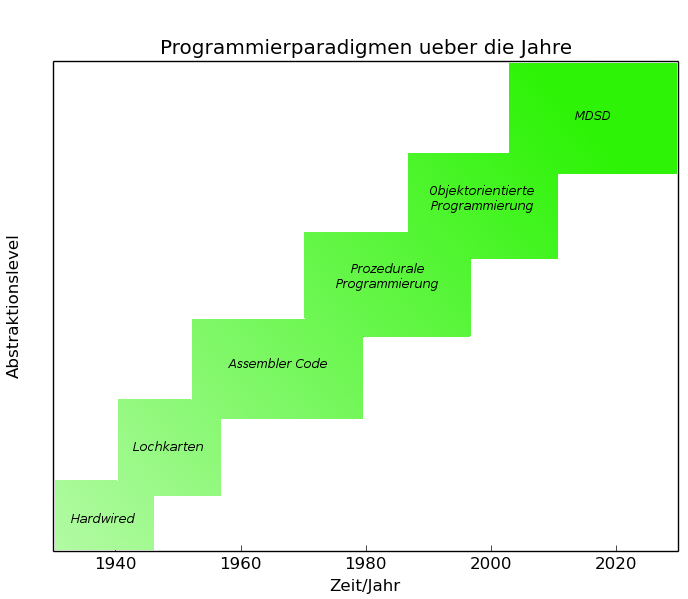
\includegraphics[width = \textwidth]{Bilder/paradigmsInTime(matplotlib).png}
		\caption{Programmierparadigmen im Verlauf der Zeit}
		\label{paradigmnsintime}
	\end{center}
\end{figure}Entwickler auf der ganzen Welt benutzen Bibliotheken und Frameworks, um bereits entwickelte Lösungen wiederverwenden zu können und um bekannte Lösungsansätze für bekannte Problemstellungen zu verwenden. Der hierbei entwickelte Code richtet sich also nach einem bereits vorgelegten Plan. Jener Quellcode, der manuell ergänzt werden muss, lässt sich nun teilweise automatisiert ergänzen.  Dieses Ziel verfolgt das \textbf{M}odel \textbf{D}riven \textbf{S}oftware \textbf{D}evelopment (\textit{MDSD}). Schematischer Code kann in domänenspezifischen Modellen verarbeitet werden. Nachdem Modelle konzipiert sind, ist es möglich automatisiert auf domänenspezifische Problemstellungen einzugehen. Im Falle der Industrie bedeutet dies Massenproduktion, ermöglicht von Robotern. In Bezug auf Softwareentwicklung, bedeutet dies Code, der Code generiert. Die Idee ist, variable Teile des Codes über ein Modell zu beschreiben. Das Programm ist selbstständig in der Lage, das Modell in den gewünschten Code umzuwandeln. Das besagte Modell kann hierbei drastisch vereinfacht, oder auf eine bestimmte Benutzerzielgruppe(Domäne) angepasst sein. Es lässt sich also problemlos einrichten, beispielsweise einem Banker über seine gewohnten Fachbegriffe eine \textbf{D}omain \textbf{S}pecific \textbf{L}anguage (\textit{DSL}) zu bieten, welche syntaktisch auch noch einer seiner Tabellen oder beispielsweise Buchungssätzen ähnelt und somit für ihn unkompliziert und sofort erlernbar ist. Für die Umwandlung eines Modells in konkreten Code (Generat) sind sogenannte Generatoren notwendig. 
\linebreak 
Siehe auch \Mycite{trompeter:mda}

\section{Was Ist MoDiGen?}\label{modigen}
Domänenspezifische Modellierung erfreut sich wachsender Beliebtheit in der Softwareentwicklung. Projekte, die für ein domänenspezifisches Problem graphische Modellierungstools benötigen, können entweder ein sehr spezifisches Tool benutzen, was nur dann möglich ist, wenn das Problem exakt durch das Tool beschrieben werden kann. Ansonsten muss ein generischer Editor herangezogen werden, doch diese sind dann in der Regel derart komplex, dass es nicht mehr möglich ist, sein Problem schnell und unkompliziert darstellen zu können. Das \textit{MoDiGen} (\textbf{Mo}del \textbf{Di}agram \textbf{Gen}erator) Projekt will es ermöglichen, durch kurze und schnell umsetzbare textuelle DSLs, graphische Editoren erzeugen zu lassen, deren Entwicklung sonst überaus zeitaufwendig sein kann. Hierfür wurde einerseits ein hoch abstrahiertes Metamodell erstellt, das komplexe Klassenhierarchien darstellen kann, außerdem wurden einige textuelle DSLs erstellt, über die die Modellklassen beschrieben werden können (Diagram, Shape, Connection, Style). So soll dem Anwender (\textit{Domain Expert}) die Möglichkeit geboten werden, eigene graphische Elemente zu erzeugen. Dabei kann es sich auch um Verbindungselemente handeln, denn diese werden im Metamodell von MoDiGen getrennt und ebenbürtig zu den eigentlichen Elementen gehandhabt (vgl. \Mycite{gerhart:modigen_concept}). Außerdem werden sie nicht wie bei etwa \textit{Ecore} nur als Attribut eines Modells gehalten. Im Hinblick auf die Skalierbarkeit ist dies vorteilhaft, da Elemente nicht über ein relationales Schema abgebildet werden müssen, um sie in einer Datenbank zu hinterlegen. Hieraus entstehen wiederum Vorteile bezüglich der Skalierbarkeit und des Datenzugriffs.
\section{Aufgabenstellung}
Hinsichtlich der Flexibilität der Modelle und der Skalierbarkeit, bieten bestehende Lösungen wie \textit{Xtext} und \textit{Ecore} derzeit keine Ideale Lösung. Die relativ junge Programmiersprache \textit{Scala} ist, wie der Name schon andeuten soll, mit einem besonderen Fokus auf die Skalierbarkeit entwickelt worden. Wie bereits in \ref{modigen} erläutert, stützt sich das MoDiGen Projekt auf ein neues, selbst entwickeltes Metamodell, welches hinsichtlich der Skalierbarkeit und der Speicherauslastung wesentlich bessere Ergebnisse erzielt. So wie das Metamodell sollen nun auch die Parser und Generatoren in Scala umgesetzt werden. Es soll untersucht werden, inwiefern Scala (als allzweckstaugliche Programmiersprache) sich dafür eignet, die Rolle bestehender spezialisierter Technologien zu übernehmen. Wo kann Scala seine Stärken spielen lassen und wo ist es den bisherigen Lösungen unterlegen? Dafür sollen u.a. MoDiGens Modellklassen: Style, Shape und Diagram in Scala umgesetzt werden und die entsprechenden Parser und Generatoren erstellt werden. Konkreter: Es müssen zunächst die geforderten Objektstrukturen geschaffen werden um Style, Shape, Connection und Diagram abbilden zu können. Hierbei muss darauf geachtet werden, dass ein Style ein weiteres Style assoziieren kann um eine Vererbung zu ermöglichen.\\\\Shapes können derzeit aufgrund der Komplexität der Modellklasse nicht vererbt werden. Sowohl die Shapevererbung als auch Mehrfachvererbung im allgemeinen ist mit bestehenden Technologien nicht möglich und soll daher auf Umsetzbarkeit mit Scala überprüft werden. Des weiteren sind die Beziehungen der Modelle untereinander genau geklärt - siehe Abbildung \ref{diagramshapestyle}. Diagrams können auf Styles und Shapes verweisen und Shapes können Styles referenzieren. Außerdem muss ein Parser erstellt werden, der in der Lage ist die \textit{Spray} DSL zu interpretieren und entsprechend der Modelle zu instantiieren. Zuletzt kommen Generatorenklassen, die schließlich entsprechende Generate aus den erzeugten Objekten erstellen können.\\\\Es handelt sich also um eine Studie zur Umsetzbarkeit von Parser- und Generatorenklassen in Scala, mit speziellem Fokus auf die Möglichkeit komplexe Vererbungshierarchien darstellen zu können. Hierbei liegt die größte Herausforderung darin, einen Parsingmechanismus zu erstellen, der mit rekursiven DSL Definitionen umgehen kann und der in der Lage ist komplexe Vererbungshierarchien zu erkennen und umzusetzen. Da der Autor Scala erst für dieses Projekt erlernt, kann davon ausgegangen werden, dass alle verwendeten Techniken anfängerfreundlich sind.
\begin{figure}[h]
\begin{center}
\includegraphics[scale = 0.7]{Bilder/vereinfachteobjektstruktur.png}
%\includegraphics[width = \textwidth]{Bilder/vereinfachteobjektstruktur.png}
\caption{Klassendiagramm Diagram, Shape, Style (Sehr stark vereinfacht)}
\label{diagramshapestyle}
\end{center}
\end{figure}